\documentclass{beamer}
%\usetheme{Boadilla}
%\usetheme{Szeged}
%\usetheme{Singapore}
%\usetheme{Frankfurt}
\usecolortheme{dove}
\setbeamertemplate{navigation symbols}{}
%\setbeamertemplate{headline}
%{%
%\vskip .1cm
%\insertsectionnavigationhorizontal{\textwidth}{}{}
%}
\newenvironment{alltt}{\ttfamily}{\par}
\usepackage{amsmath,amssymb,amsfonts,amsthm, multicol, subfigure, color}
\usepackage{bm}
\usepackage{graphicx}
\usepackage{tabularx}
\usepackage{booktabs}
\usepackage{hyperref}
\usepackage{pdfpages}
\usepackage{xcolor}
\definecolor{dodgerblue}{rgb}{.118, .575, 1}
\definecolor{seagreen4}{RGB}{46, 139, 87}
\def\independenT#1#2{\mathrel{\rlap{$#1#2$}\mkern2mu{#1#2}}}
\newcommand\independent{\protect\mathpalette{\protect\independenT}{\perp}}
\newcommand\indep{\protect\mathpalette{\protect\independenT}{\perp}}
\def\logit{\text{logit}}
\usepackage{stackrel}
\usepackage{tikz}
\usetikzlibrary{arrows,shapes.arrows,positioning,shapes,patterns,calc}
\newcommand\slideref[1]{\vskip .1cm \scriptsize \textcolor{gray}{{#1}}}
\definecolor{seagreen}{RGB}{46, 139, 87}
\newcommand\red[1]{\color{red}#1}
\newcommand\blue[1]{\color{blue}#1}
\newcommand\gray[1]{\color{gray}#1}
\newcommand\green[1]{\color{olive}#1}
\newcommand\seagreen[1]{\color{seagreen}#1}
\newcommand\purple[1]{\color{purple}#1}
\newcommand\orange[1]{\color{orange}#1}
\newcommand\black[1]{\color{black}#1}
\newcommand\white[1]{\color{white}#1}
\newcommand\teal[1]{\color{teal}#1}
\newcommand\magenta[1]{\color{magenta}#1}
\newcommand\Fuchsia[1]{\color{Fuchsia}#1}
\newcommand\BlueGreen[1]{\color{BlueGreen}#1}
\newcommand\bblue[1]{\textcolor{blue}{\textbf{#1}}}
\newcommand\bred[1]{\textcolor{red}{\textbf{#1}}}
\newcommand\bgray[1]{\textcolor{gray}{\textbf{#1}}}
\newcommand\bgreen[1]{\textcolor{seagreen}{\textbf{#1}}}
\colorlet{lightgray}{gray!40}
\pgfdeclarelayer{bg}    % declare background layer for tikz
\pgfsetlayers{bg,main} % order layers for tikz
\newcommand\bref[2]{\href{#1}{\color{blue}{#2}}}
\newcommand\mycite[1]{\begin{scriptsize}\textcolor{darkgray}{(#1)}\end{scriptsize}}
\newcommand\iid{\stackrel{\text{iid}}{\sim}}
\newcommand\E{\text{E}}
\newcommand\V{\text{V}}
\renewcommand\P{\text{P}}
\newcommand{\Cov}{\text{Cov}}
\newcommand{\Cor}{\text{Cor}}
\newcommand\doop{\text{do}}
\newcommand{\tcframe}{\frame{
\small{
\only<1|handout:0>{\tableofcontents}
\only<2|handout:1>{\tableofcontents[currentsection]}}
}}
% Credit for the following to https://tex.stackexchange.com/questions/44983/beamer-removing-headline-and-its-space-on-a-single-frame-for-plan-but-keepin
\makeatletter
    \newenvironment{withoutheadline}{
        \setbeamertemplate{headline}[default]
        \def\beamer@entrycode{\vspace*{-\headheight}}
    }{}
\makeatother
\setbeamercovered{invisible}
\usepackage[round]{natbib}
\bibliographystyle{humannat-mod}
\setbeamertemplate{enumerate items}[default]
\usepackage{mathtools}
% BELOW THREE LINES MAKES NAME IN FOOTER
\setbeamertemplate{footline}[text line]{%
\parbox{\linewidth}{\vspace*{-8pt}Lundberg, Johnson, and Stewart. Setting the Target: Precise Estimands and the Gap Between Theory and Empirics}}%\hfill\insertshortauthor\hfill\insertpagenumber}}
%t\setbeamertemplate{navigation symbols}{}

% Make the header figure that will appear frequently
\newcommand\headerfigure{
\begin{tikzpicture}[x = \textwidth, y = \textheight, every node/.style={anchor = center}]
\node at (0,1) {\resizebox{\textwidth}{!}{\begin{tikzpicture}[x = 1.7in, y = .3in]
    \node[cloud, draw, align=center, cloud puffs=20,cloud puff arc=110, aspect=2, inner sep=.5mm, font = \small] (general) at (-.1,0) {Theory or\\general goal};
    %%%%%%%%%%
    \node[align=center, font = \small] (theoretical) at (1,0) {Theoretical\\estimands};
    \draw[->, thick] (general) -- (theoretical);
    \node[align = center, anchor = south, font = {\bf\small}] at (.5,0) {Set};
    \node[align = center, anchor = north, font = \small] at (.5,0) {by argument};
    %%%%%%%%%%
    \node[align=center, font = \small] (empirical) at (2,0) {Empirical\\estimands};
    \draw[->, thick] (theoretical) -- (empirical);
    \node[align = center, anchor = south, font = {\bf\small}] at (1.5,0) {Link};
    \node[align = center, anchor = north, font = \small] at (1.5,0) {by assumption};
    %%%%%%%%%%
    \node[align=center, font = \small] (estimate) at (3,0) {Estimation\\strategies};
    \draw[->, thick] (empirical) -- (estimate);
    \node[align = center, anchor = south, font = {\bf\small}] at (2.5,0) {Learn};
    \node[align = center, anchor = north, font = \small] at (2.5,0) {by data};
    \end{tikzpicture}
    }};
\end{tikzpicture}
}
% Make the versions that have only one step in black
\newcommand\headerfigureset{
\begin{tikzpicture}[x = \textwidth, y = \textheight, every node/.style={anchor = center}]
\node at (0,1) {\resizebox{\textwidth}{!}{\begin{tikzpicture}[x = 1.7in, y = .3in]
    \node[cloud, draw, gray, align=center, cloud puffs=20,cloud puff arc=110, aspect=2, inner sep=.5mm, font = \small] (general) at (-.1,0) {Theory or\\general goal};
    \draw[line width = 2pt, seagreen] (.22,-.75) -- (1.2,-.75);
    %%%%%%%%%%
    \node[align=center, font = \small] (theoretical) at (1,0) {Theoretical\\estimands};
    \draw[->, thick] (general) -- (theoretical);
    \node[align = center, anchor = south, font = {\bf\small}] at (.5,0) {Set};
    \node[align = center, anchor = north, font = \small] at (.5,0) {by argument};
    %%%%%%%%%%
    \node[align=center, font = \small, gray] (empirical) at (2,0) {Empirical\\estimands};
    \draw[->, thick, gray] (theoretical) -- (empirical);
    \node[align = center, anchor = south, font = {\bf\small}, gray] at (1.5,0) {Link};
    \node[align = center, anchor = north, font = \small, gray] at (1.5,0) {by assumption};
    %%%%%%%%%%
    \node[align=center, font = \small, gray] (estimate) at (3,0) {Estimation\\strategies};
    \draw[->, thick, gray] (empirical) -- (estimate);
    \node[align = center, anchor = south, font = {\bf\small}, gray] at (2.5,0) {Learn};
    \node[align = center, anchor = north, font = \small, gray] at (2.5,0) {by data};
    \end{tikzpicture}
    }};
\end{tikzpicture}
}
\newcommand\headerfigurelink{
\begin{tikzpicture}[x = \textwidth, y = \textheight, every node/.style={anchor = center}]
\node at (0,1) {\resizebox{\textwidth}{!}{\begin{tikzpicture}[x = 1.7in, y = .3in]
    \node[gray, cloud, draw, align=center, cloud puffs=20,cloud puff arc=110, aspect=2, inner sep=.5mm, font = \small] (general) at (-.1,0) {Theory or\\general goal};
    \draw[line width = 2pt, seagreen] (1.2,-.75) -- (2.2,-.75);
    %%%%%%%%%%
    \node[align=center, font = \small, gray] (theoretical) at (1,0) {Theoretical\\estimands};
    \draw[->, thick, gray] (general) -- (theoretical);
    \node[align = center, anchor = south, font = {\bf\small}, gray] at (.5,0) {Set};
    \node[align = center, anchor = north, font = \small, gray] at (.5,0) {by argument};
    %%%%%%%%%%
    \node[align=center, font = \small] (empirical) at (2,0) {Empirical\\estimands};
    \draw[->, thick] (theoretical) -- (empirical);
    \node[align = center, anchor = south, font = {\bf\small}] at (1.5,0) {Link};
    \node[align = center, anchor = north, font = \small] at (1.5,0) {by assumption};
    %%%%%%%%%%
    \node[align=center, font = \small, gray] (estimate) at (3,0) {Estimation\\strategies};
    \draw[->, thick, gray] (empirical) -- (estimate);
    \node[align = center, anchor = south, font = {\bf\small}, gray] at (2.5,0) {Learn};
    \node[align = center, anchor = north, font = \small, gray] at (2.5,0) {by data};
    \end{tikzpicture}
    }};
\end{tikzpicture}
}
\newcommand\headerfigurelearn{
\begin{tikzpicture}[x = \textwidth, y = \textheight, every node/.style={anchor = center}]
\node at (0,1) {\resizebox{\textwidth}{!}{\begin{tikzpicture}[x = 1.7in, y = .3in]
    \node[gray, cloud, draw, align=center, cloud puffs=20,cloud puff arc=110, aspect=2, inner sep=.5mm, font = \small] (general) at (-.1,0) {Theory or\\general goal};
    \draw[line width = 2pt, seagreen] (2.2,-.75) -- (3.2,-.75);
    %%%%%%%%%%
    \node[align=center, font = \small, gray] (theoretical) at (1,0) {Theoretical\\estimands};
    \draw[->, thick, gray] (general) -- (theoretical);
    \node[align = center, anchor = south, font = {\bf\small}, gray] at (.5,0) {Set};
    \node[align = center, anchor = north, font = \small, gray] at (.5,0) {by argument};
    %%%%%%%%%%
    \node[align=center, font = \small, gray] (empirical) at (2,0) {Empirical\\estimands};
    \draw[->, thick, gray] (theoretical) -- (empirical);
    \node[align = center, anchor = south, font = {\bf\small}, gray] at (1.5,0) {Link};
    \node[align = center, anchor = north, font = \small, gray] at (1.5,0) {by assumption};
    %%%%%%%%%%
    \node[align=center, font = \small] (estimate) at (3,0) {Estimation\\strategies};
    \draw[->, thick] (empirical) -- (estimate);
    \node[align = center, anchor = south, font = {\bf\small}] at (2.5,0) {Learn};
    \node[align = center, anchor = north, font = \small] at (2.5,0) {by data};
    \end{tikzpicture}
    }};
\end{tikzpicture}
}

\title{\blue{Estimands in the study of inequality}}
\author{Ian Lundberg}
\date{Stewart Lab\\Princeton University\\7 October 2019}
%\date{Notestein Seminar\\Office of Population Research\\Princeton University\\15 October 2019}

\begin{document}

%\frame{\titlepage}

\begin{frame}
\centering
\begin{tikzpicture}[x = .5\textwidth, y = .5\textwidth]
\node at (-1,-1) {};
\node at (1,1) {};
\node[font = \huge, align = left, anchor = north west, blue] at (-1, .9) {\textbf{Setting the Target}};
\node[font = \LARGE, align = left, anchor = north west] at (-1,.7) {Precise Estimands\\and the Gap Between\\Theory and Empirics};
\node[anchor = north east] at (1,1) {
\includegraphics[width = 1.3in]{output/target}};
%\node[anchor = north east] at (1, .9) {4 August 2020};
%\node[anchor = north east, align = right] at (1, .8) {Annual Meeting of the\\American Sociological\\Association};
\node[align = center, anchor = south west, align = left] (ian) at (-1, .05) {Ian Lundberg};
\node[align = center, anchor = south] (rebecca) at (-.05,.05) {Rebecca Johnson};
\node[align = center, anchor = south west] (brandon) at (.3, .05) {Brandon M. Stewart};
\node[align = left, anchor = north west, font = \scriptsize] (ianAffil) at (ian.south west) {Princeton Sociology\\ilundberg@princeton.edu};
\node[align = center, anchor = north, font = \scriptsize] (rebeccaAffil) at (rebecca.south) {Dartmouth Quantitative\\Social Science\\rebecca.ann.johnson\\@dartmouth.edu};
\node[align = right, anchor = north east, font = \scriptsize] (brandonAffil) at (brandon.south east) {Princeton Sociology\\bms4@princeton.edu};
\node[align = left, anchor = south west, font = \scriptsize, text width = \textwidth] at (-1, -.65) {4 August 2020. Annual Meeting of the American Sociological Association.\\Paper on SocArxiv [\bref{https://doi.org/10.31235/osf.io/ba67n}{link}]. Replication code on GitHub [\bref{https://github.com/ilundberg/replication/tree/master/setting_the_target}{link}]. Slides on GitHub [\bref{https://github.com/ilundberg/slides}{link}]. Research reported in this publication was supported by The Eunice Kennedy Shriver National Institute of Child Health \& Human Development of the National Institutes of Health under Award Number P2CHD047879.};
\end{tikzpicture}
\end{frame}

\section{Intro}

\begin{frame}{\bblue{State of the field:} How methods are used in sociology}
%\textbf{Theory equated with coefficients}\vskip .1in
\pause
\begin{center}``[Variables] empirically perform as \textcolor{blue}{theoretically predicted},\\ \pause by displaying statistically significant\\\textcolor{blue}{effects net of other variables} in the right direction''
\end{center}
\end{frame}

\begin{frame}
\begin{tikzpicture}[x = \textwidth, y = \textheight]
\node at (0,0) {};
\node at (1,1) {};
\node[anchor = north west] at (0,.9) {The \bblue{target tautology}:};
\node[anchor = north, font = \small] (t1) at (.5, .8) {Research goals are defined by hypotheses about model coefficients};
\node<2->[anchor = north, font = \small] (t2) at (.5, .7) {The goal is only defined within the statistical model};
\draw<2->[->, thick] (t1) -- (t2);
\node<3->[anchor = north, font = \small] (t3) at (.5, .6) {It becomes impossible to reason about other estimation strategies};
\draw<3->[->, thick] (t2) -- (t3);
\node<4->[anchor = north west] at (0,.4) {\bblue{Solution}:};
\node<4->[anchor = north, align = center, font = \small] at (.5,.3) {State the research goal\\separately from the estimation strategy};
\node<5->[anchor = south east, align = right, font = \footnotesize] at (1,.35) {Our \bgreen{diagnosis} for the source\\of many methodological problems};
\draw<5->[->, thick, seagreen] (.8, .35) to[out = 270, in = 0] (.68,.27);
\end{tikzpicture}
\end{frame}

\begin{frame}{Our solution: A framework centered on \bblue{estimands}}
{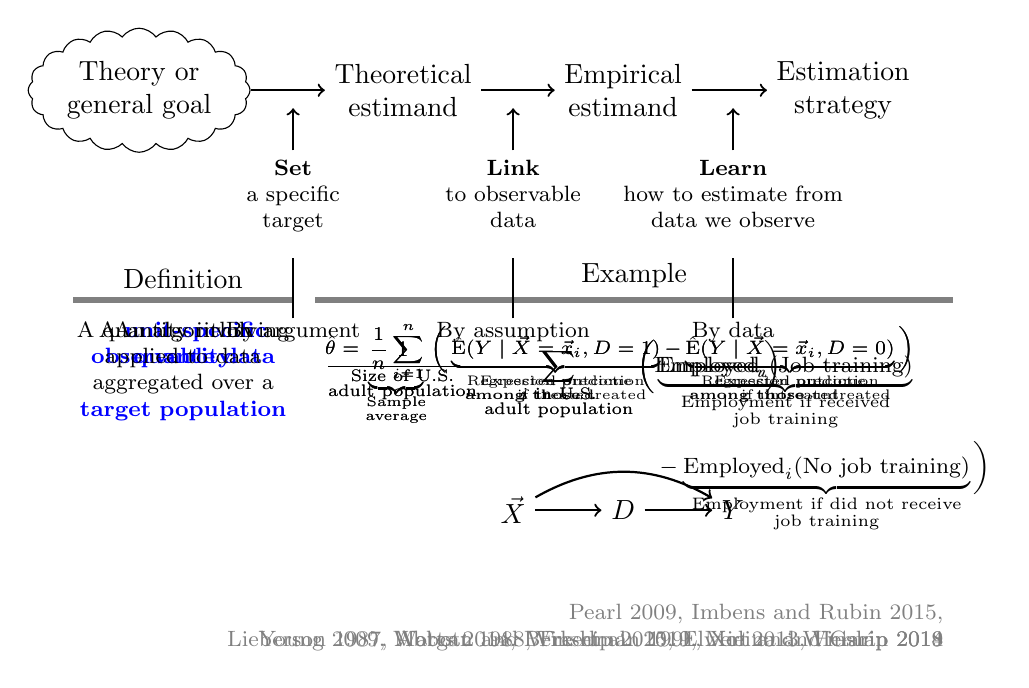
\begin{tikzpicture}[x = 1.1in, y = .3in]
    \node[cloud, draw, align=center, cloud puffs=20,cloud puff arc=110, aspect=2, inner sep=.5mm] (general) at (-.2,0) {Theory or\\general goal};
    \node[align=center, white] (theoretical) at (1,0) {Theoretical\\estimand};
    \node[align=center, white] (empirical) at (2,0) {Empirical\\estimand};
    \node[align=center] (estimate) at (3,0) {Estimation\\strategy};
    \draw[->, thick] (general) -- (theoretical);
    \draw[->, thick] (theoretical) -- (empirical);
    \draw[->, thick] (empirical) -- (estimate);
    %%%%%%%%%%
    \node<2->[align=center] (theoretical) at (1,0) {Theoretical\\estimand};
    \node<2->[align=center, font = \footnotesize, anchor = north] (define) at (.5,-1) {\textbf{Set}\\a specific\\target};
    %\node[align=center, font = \scriptsize, anchor = north west] at (-.6,-5.4) {\textbf{Example tools:}};
    %\node[align=center, font = \scriptsize, anchor = north] at (.5,-5.4) {Target population,\\Causal contrast};
    \draw<2->[->, thick] (define) -- (.5,-.3);
    %\draw[thick] (.5,-5.3) -- (.5,-4.5);
    \draw<3-14>[line width = 2pt, gray] (-.5,-3.5) -- node[midway, above, text = black] {Definition} (.5,-3.5);
     \node<3-6>[align = center, rounded corners, font = \footnotesize, anchor = north, text width = 1.1in] at (0, -3.7) {A \bblue{unit-specific quantity}\\aggregated over a\\\bblue{target population}};
    \draw<4-14>[line width = 2pt, gray] (.6,-3.5) -- node[midway, above, text = black] {Example} (3.5,-3.5);
     \node<4>[anchor = north west, font = \footnotesize] at (.6,-4) {$\begin{aligned}\frac{1}{\substack{\text{Size of U.S.}\\\text{adult population}}}\sum_{\substack{i\text{ in U.S.}\\\text{adult population}}}\bigg(\text{Employed}_i\bigg)\end{aligned}$};
     \node<5-6>[anchor = north west, font = \footnotesize] at (.6,-4) {$\begin{aligned}\frac{1}{\substack{\text{Size of U.S.}\\\text{adult population}}}\sum_{\substack{i\text{ in U.S.}\\\text{adult population}}} \bigg(&\underbrace{\text{Employed}_i(\text{Job training})}_{\substack{\text{Employment if received}\\\text{job training}}} \\ &- \underbrace{\text{Employed}_i(\text{No job training})}_{\substack{\text{Employment if did not receive}\\\text{job training}}}\bigg) \end{aligned}$};
    \node<6>[align=right, gray, font = \footnotesize, anchor = south east] (define) at (3.5,-9.5) {Lieberson 1987, Abbott 1988, Freedman 1991, Xie 2013, Hern\'an 2018};
    %%%%%%%%%%
    \node<7->[align=center] (empirical) at (2,0) {Empirical\\estimand};
    \node<7->[align=center, font = \footnotesize, anchor = north] (identify) at (1.5,-1) {\textbf{Link}\\to observable\\data};
    %\node[align=center, font = \footnotesize, anchor = north] at (1.5,-5.4) {Directed Acyclic Graphs,\\Potential outcomes};
    \draw<7->[->, thick] (identify) -- (1.5,-.3);
     \node<8-10>[align = center, rounded corners, font = \footnotesize, anchor = north, text width = 1.1in] at (0, -3.7) {A quantity involving \bblue{observable data}};
      \node<9-10>[anchor = north west, font = \scriptsize] at (.6,-3.7) {$\begin{aligned}\theta &= \underbrace{\frac{1}{n}\sum_{i=1}^n}_{\substack{\text{Sample}\\\text{average}}} \bigg(\underbrace{\E(Y\mid \vec{X} = \vec{x}_i, D = 1)}_{\substack{\text{Expected outcome}\\\text{\textbf{among those} treated}}} - \underbrace{\E(Y\mid \vec{X} = \vec{x}_i, D = 0)}_{\substack{\text{Expected outcome}\\\text{\textbf{among those} untreated}}}\bigg)\end{aligned}$};
      \node<9-10> (x) at (1.5,-7) {$\vec{X}$};
      \node<9-10> (d) at (2,-7) {$D$};
      \node<9-10> (y) at (2.5,-7) {$Y$};
      \draw<9-10>[->, thick] (x) -- (d);
      \draw<9-10>[->, thick] (x) to[bend left] (y);
      \draw<9-10>[->, thick] (d) -- (y);
    \node<10>[align=right, gray, font = \footnotesize, anchor = south east] (define) at (3.5,-9.5) {Pearl 2009, Imbens and Rubin 2015,\\Morgan and Winship 2015, Elwert and Winship 2014};
    %%%%%%%%%%
    \node<11->[align=center, font = \footnotesize, anchor = north] (learn) at (2.5,-1) {\textbf{Learn}\\how to estimate from\\data we observe};
    %\node[align=center, font = \footnotesize, anchor = north] at (2.5,-5.4) {OLS regression,\\Machine learning};
    \draw<11->[->, thick] (learn) -- (2.5,-.3);
    %\draw[thick] (2.5,-5.3) -- (2.5,-4.5);
     \node<12-14>[align = center, rounded corners, font = \footnotesize, anchor = north, text width = 1.1in] at (0, -3.7) {An algorithm applied to data};
    \node<13-14>[anchor = north west, font = \scriptsize] at (.6,-3.7) {$\begin{aligned}%\theta &= \underbrace{\frac{1}{n}\sum_{i=1}^n}_{\substack{\text{Sample}\\\text{average}}} \bigg(\underbrace{\E(Y\mid \vec{X} = \vec{x}_i, D = 1)}_{\substack{\text{Expected outcome}\\\text{\textbf{among those} treated}}} - \underbrace{\E(Y\mid \vec{X} = \vec{x}_i, D = 0)}_{\substack{\text{Expected outcome}\\\text{\textbf{among those} untreated}}}\bigg) \\
    \hat\theta &= \underbrace{\frac{1}{n}\sum_{i=1}^n}_{\substack{\text{Sample}\\\text{average}}} \bigg(\underbrace{\hat\E(Y\mid \vec{X} = \vec{x}_i, D = 1)}_{\substack{\text{Regression prediction}\\\text{if treated}}} - \underbrace{\hat\E(Y\mid \vec{X} = \vec{x}_i, D = 0)}_{\substack{\text{Regression prediction}\\\text{if untreated}}}\bigg)\end{aligned}$};
    \node<14>[align=right, gray, font = \footnotesize, anchor = south east] (define) at (3.5,-9.5) {Young 2009, Watts 2014, Berk et al. 2019, Molina and Garip 2019};
    % Types of argument
    \onslide<15>{
    \node[align=center, font = \footnotesize, anchor = north] at (.5,-3.7) {By argument};
    \draw[thick] (.5,-3.8) -- (.5,-2.8);
    \node[align=center, font = \footnotesize, anchor = north] at (1.5,-3.7) {By assumption};
    \draw[thick] (1.5,-3.8) -- (1.5,-2.8);
    \node[align=center, font = \footnotesize, anchor = north] at (2.5,-3.7) {By data};
    \draw[thick] (2.5,-3.8) -- (2.5,-2.8);
    }
    \end{tikzpicture}
    }
\end{frame}

\begin{frame}[t]
\headerfigure
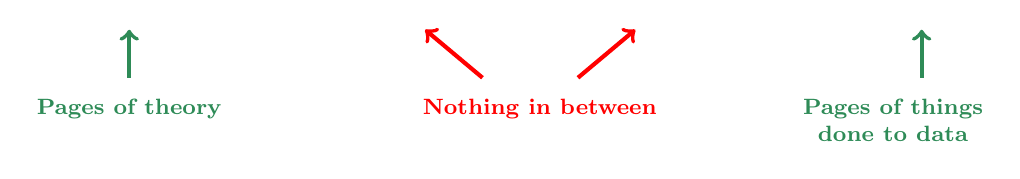
\begin{tikzpicture}[x = \textwidth, y = .3in]
\node<2->[anchor = north, align = center, font = {\bf\footnotesize}, seagreen] at (.1,0) {Pages of theory};
\draw<2->[->, seagreen, line width = 1.5pt] (.1,.2) -- (.1,1);
\node<3->[anchor = north, align = center, font = {\bf\footnotesize}, seagreen] at (.9,0) {Pages of things\\done to data};
\draw<3->[->, seagreen, line width = 1.5pt] (.93,.2) -- (.93,1);
\node<4->[anchor = north, align = center, font = {\bf\footnotesize}, red] at (.53,0) {Nothing in between};
\draw<4->[->, red, line width = 1.5pt] (.47,.2) -- (.41,1);
\draw<4->[->, red, line width = 1.5pt] (.57,.2) -- (.63,1);
\end{tikzpicture}
\end{frame}

\begin{frame}[t]
\headerfigureset
\resizebox{\textwidth}{!}{
    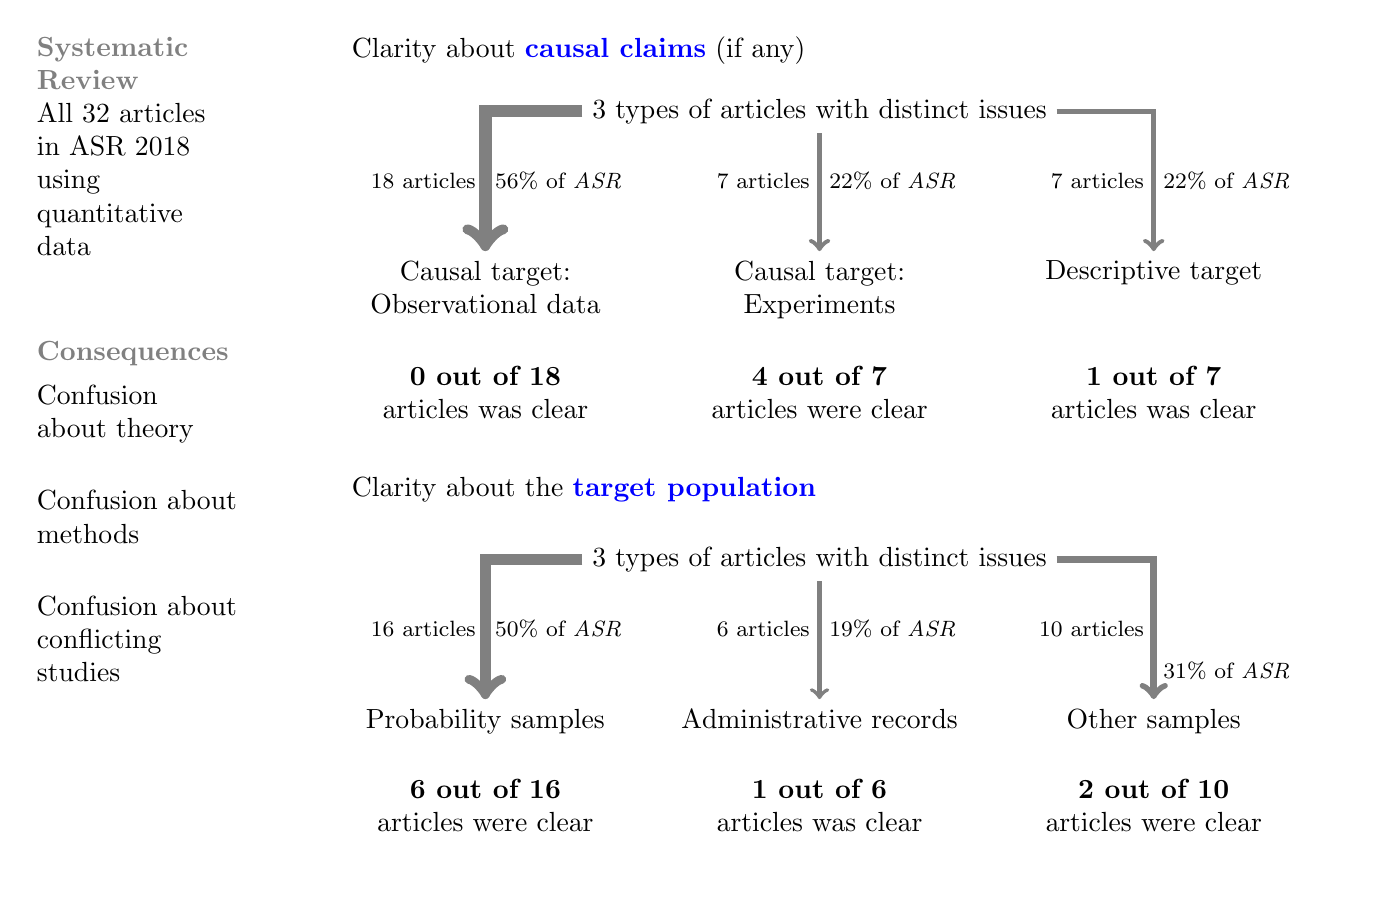
\begin{tikzpicture}[x = \textwidth, y = .7in]
    \node at (1.05,-6.5) {};
    %\draw[line width = 1.5pt] (asr.south west) -- (asr.south east);
    \node[align = left, anchor = north east, text width = 1in] (asr) at (-.1,-.4) {\bgray{Systematic Review}\\All 32 articles\\in ASR 2018\\using\\quantitative\\data};
    \node<2->[align = left, anchor = north west] at (0,-.4) {Clarity about \bblue{causal claims} (if any)};
    %\node[align = right, anchor = east] at (1,-.6) {Details in Appendix Table \ref{tab:causal_contrast_overview}};
    \node<4->[align = center] (three) at (.5,-1) {3 types of articles with distinct issues};
    \node<4->[align = center, anchor = north] (causal_observational) at (.15,-2) {Causal target:\\Observational data};
    \node<4->[align = center, anchor = north] (descriptive) at (.85,-2) {Descriptive target};
    \node<4->[align = center, anchor = north] (causal_experiments) at (.5,-2) {Causal target:\\Experiments};
    % Line widths are the percent multiplied by 8
    \draw<4->[->, line width = 4.48pt, gray] (three) -- (.15,-1) -- (causal_observational);
    \draw<4->[->, line width = 1.76pt, gray] (three) -- (causal_experiments);
    \draw<4->[->, line width = 1.76pt, gray] (three) -- (.85,-1) -- (descriptive);
    \node<4->[font = \footnotesize, anchor = east, align = right] at (.15,-1.5) {18 articles};
    \node<4->[font = \footnotesize, anchor = east, align = right] at (.5,-1.5) {7 articles};
    \node<4->[font = \footnotesize, anchor = east, align = right] at (.85,-1.5) {7 articles};
    \node<4->[font = \footnotesize, anchor = west, align = left] at (.15,-1.5) {56\% of \emph{ASR}};
    \node<4->[font = \footnotesize, anchor = west, align = left] at (.5,-1.5) {22\% of \emph{ASR}};
    \node<4->[font = \footnotesize, anchor = west, align = left] at (.85,-1.5) {22\% of \emph{ASR}};
    \node<5->[anchor = north, align = center] at (.15,-2.75) {\textbf{0 out of 18}\\articles was clear};
    \node<6->[anchor = north, align = center] at (.5,-2.75) {\textbf{4 out of 7}\\articles were clear};
    \node<7->[anchor = north, align = center] at (.85,-2.75) {\textbf{1 out of 7}\\articles was clear};
    %%%%%%%%%%%%%%%%%%%%%%%%%%%%%%%%%%
    \node<3->[anchor = west, align = left] at (0,-3.7) {Clarity about the \bblue{target population}};
    \node<8->[align = center] (three_target) at (.5,-4.2) {3 types of articles with distinct issues};
    \node<8->[align = center, anchor = north] (probability_samples) at (.15,-5.2) {Probability samples};
    \node<8->[align = center, anchor = north] (administrative_records) at (.5,-5.2) {Administrative records};
    \node<8->[align = center, anchor = north] (other_samples) at (.85,-5.2) {Other samples};
    \draw<8->[->, line width = 4pt, gray] (three_target) -- (.15,-4.2) -- (probability_samples);
    \draw<8->[->, line width = 1.5pt, gray] (three_target) -- (administrative_records);
    \draw<8->[->, line width = 2.48pt, gray] (three_target) -- (.85,-4.2) -- (other_samples);
    \node<8->[font = \footnotesize, anchor = east, align = right] at (.15,-4.7) {16 articles};
    \node<8->[font = \footnotesize, anchor = east, align = right] at (.5,-4.7) {6 articles};
    \node<8->[font = \footnotesize, anchor = east, align = right] at (.85,-4.7) {10 articles};
    \node<8->[font = \footnotesize, anchor = west, align = left] at (.15,-4.7) {50\% of \emph{ASR}};
    \node<8->[font = \footnotesize, anchor = west, align = left] at (.5,-4.7) {19\% of \emph{ASR}};
    \node<8->[font = \footnotesize, anchor = west, align = left] at (.85,-5) {31\% of \emph{ASR}};
    \node<9->[anchor = north, align = center] at (.15,-5.7) {\textbf{6 out of 16}\\articles were clear};
    \node<10->[anchor = north, align = center] at (.5,-5.7) {\textbf{1 out of 6}\\articles was clear};
    \node<11->[anchor = north, align = center] at (.85,-5.7) {\textbf{2 out of 10}\\articles were clear};
    %\node<12->[align = left, fill = white, draw = gray, line width = 2pt, rounded corners] at (.5,-3.5) {Lack of clarity\\--- Not clear what a study has shown\\--- How evidence informs theory is vague\\--- Not clear why results differ across studies};
    \node<12->[align = left, anchor = north west, text width = 1.1in] (consequences) at (asr.south west) {\textcolor{white}{filler}\\\textcolor{white}{filler}\\\bgray{Consequences}\\};
    \node<13->[align = left, anchor = north west, text width = 1in] (c1) at (consequences.south west) {Confusion about theory\\\textcolor{white}{fill}};
    \node<14->[align = left, anchor = north west, text width = 1.1in] (c2) at (c1.south west) {Confusion about methods\\\textcolor{white}{fill}};
    \node<15->[align = left, anchor = north west, text width = 1.1in] (c3) at (c2.south west) {Confusion about\\conflicting\\studies};
    \end{tikzpicture}}
    \end{frame}

%%%%%%%%%%%%%%%%%
\section{Theoretical Estimand}
%%%%%%%%%%%%%%%%%

\begin{frame}[t]
\headerfigureset 
\begin{tikzpicture}[x = \textwidth, y = .8\textheight]
\node at (0,1) {};
\node[anchor = south east, gray] at (1,.02) {Angrist and Evans 1998};
\node<2->[font = \footnotesize, align = center] (z) at (.25,.87) {First two births\\are the same sex};
\node<3->[font = \footnotesize] (t) at (.5,.87) {Third birth};
\draw<3->[->, thick] (z) -- (t);
\node<4->[font = \footnotesize] (y) at (.7,.87) {Employed};
\node<4->[font = \footnotesize, anchor = north] (u) at (.6,1) {$U$};
\draw<4->[->, thick] (t) -- (y);
\draw<4->[->, thick] (u) -- (y);
\draw<4->[->, thick] (u) -- (t);
\node<5->[anchor = west] at (0,.75) {Target population is limited:};
\node<6->[anchor = west] at (0,.68) {--- At most 53\% of mothers have 2+ children};
\node<7->[anchor = west] at (0,.61) {--- The complier population is at most 7\%};
\node<8->[anchor = west] at (0,.54) {--- Target population: at most 53\% $\times$ 7\% = 4\% of mothers};
\node<9->[anchor = west] at (0,.45) {Causal contrast is limited:};
\node<9->[anchor = west] at (0,.38) {--- Having 3 vs.~2 children};
\end{tikzpicture}
\end{frame}

\begin{frame}[t]
\headerfigureset
\begin{tikzpicture}[x = \textwidth, y = .8\textheight]
\node at (0,.5) {};
\node at (1,0) {};
\node<1->[anchor = west, gray, font = \bf] at (0,.39) {Vague statement};
\node<1->[anchor = north west, font = \small, align = left] at (0, .35) {Effect of motherhood\\on employment};
\node<2->[anchor = west, gray, font = \bf] at (.37,.39) {Precise statement};
\node<3->[anchor = north west, text width = .6\textwidth, font = \small, align = left] (precise1) at (.37,.35) {Effect of having \bblue{3 vs.~2 children}};
\node<3->[anchor = south east, font = {\bf\footnotesize}, blue, align = center] (contrast) at (1,.37) {causal\\contrast};
\draw<3->[->, line width = 2pt, blue] (contrast) to[out = 180, in = 90] (.77,.34);
\node<4->[anchor = north west, text width = .6\textwidth, font = \small, align = left] at (.37, .29) {among those with at least two children who would have a third birth if and only if the first two were of the same sex};
\node<4->[anchor = south, font = {\bf\footnotesize}, seagreen] (population) at (.15,.05) {target population};
\draw<4->[->, line width = 2pt, seagreen] (population) to[out = 90, in = 180] (.35,.2);
\draw<4->[line width = 2pt, seagreen] (.38, .28) -- (.36, .28) -- (.36, .12) -- (.38,.12);
\draw<4->[line width = 2pt, seagreen] (.97, .28) -- (.99, .28) -- (.99, .12) -- (.97,.12);
\node<5->[anchor = west] at (0, -.1) {Not just problems with instruments.};
\node<6->[anchor = west] at (0, -.18) {--- Causal contrast is vague when the treatment is continuous};
\node<7->[anchor = west] at (0, -.26) {--- Target population is vague if there are issues of common support};
\end{tikzpicture}
\end{frame}

\section{Empirical Estimand}

\begin{frame}[t]
\only<1>{\headerfigureset}
\only<2->{\headerfigurelink}
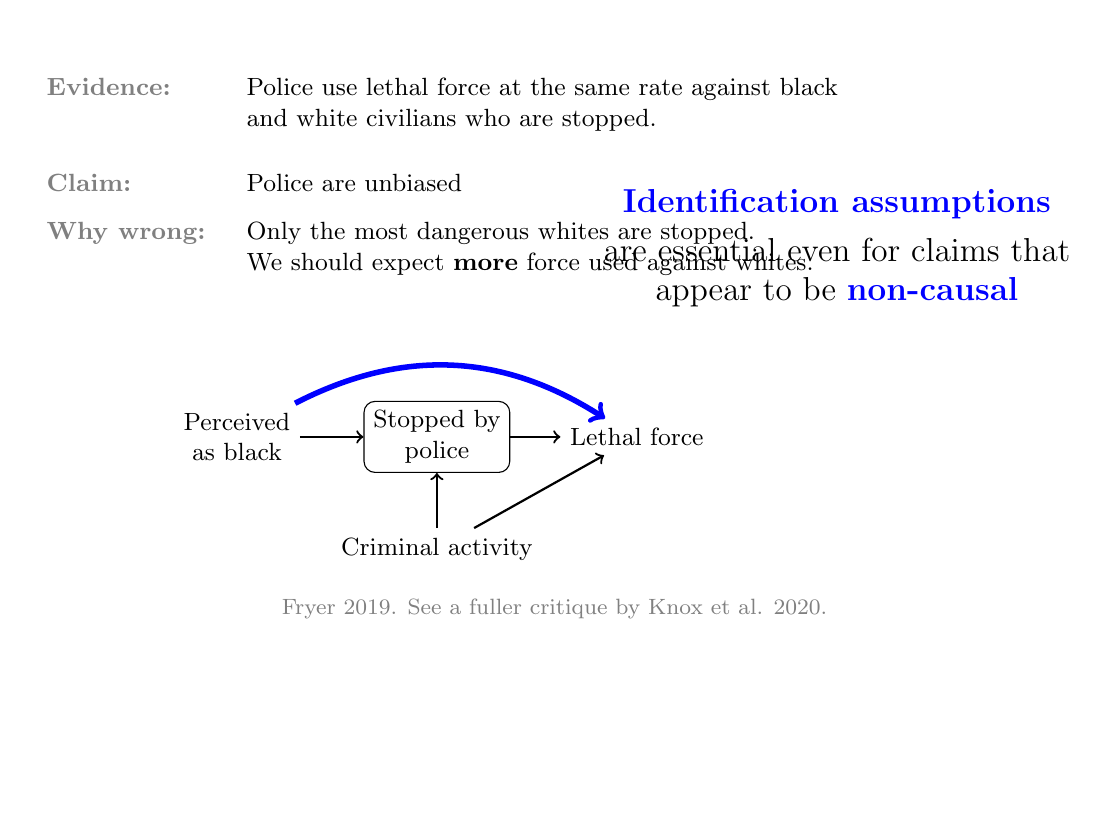
\begin{tikzpicture}[x = 1in, y = .8in]
\node at (2,-2.5) {};
\node at (0,2.2) {};
\node<3-4>[align = center, font = \large, anchor = south] at (2,1) {\bblue{Identification assumptions}};
\node<4>[align = center, font = \large, anchor = north] at (2,1) {are essential even for claims that\\appear to be \bblue{non-causal}};
    \node<5-9> at (-2,2) {};
    \node<6-9>[anchor = north west, font = {\bf\small}, gray, align = left] at (-2,2) {Evidence:};
    \node<7-9>[anchor = north west, gray, font = {\bf\small}, align = left] at (-2,1.4) {Claim:};
    \node<8-9>[anchor = north west, gray, font = {\bf\small}, align = left] at (-2,1.1) {Why wrong:};
    % Fryer
    \node<6-9>[anchor = north west, text width = 3in, font = {\small}] at  (-1, 2) {Police use lethal force at the same rate against black and white civilians who are stopped.};
    \node<7-9>[anchor = north west, text width = 3in, font = {\small}] at  (-1,1.4) {Police are unbiased};
    \node<8-9>[anchor = north west, text width = 3in, font = {\small}] at  (-1,1.1) {Only the most dangerous whites are stopped.\\We should expect \textbf{more} force used against whites.};
\node<5-9>[anchor = south east, gray, font = \footnotesize] at (2,-1.5) {Fryer 2019. See a fuller critique by Knox et al. 2020.};
    \node<9>[anchor = center, align = center, font = \small] (d) at (-1,-.3) {Perceived\\as black};
    \node<9>[anchor = center, font = \small] (u) at (0,-1) {Criminal activity};
    \node<9>[anchor = center, align=center, draw, rounded corners, font = \small] (c) at (0,-.3) {Stopped by\\police};
    \node<9>[anchor = center, align=center, font = \small] (y) at (1,-.3) {Lethal force};    
    \draw<9>[->, thick] (d) -- (c);
    \draw<9>[->, thick] (c) -- (y);
    \draw<9>[->, thick] (u) -- (c);
    \draw<9>[->, thick] (u) -- (y);
    \draw<9>[->, blue, line width = 2pt] (d) to[bend left] (y);
    \end{tikzpicture}
    \end{frame}

\section{Estimation}

\begin{frame}[t]
\headerfigurelearn \centering
A \bblue{statistical model} enters here (and only here)
\end{frame}

% PAL AND WALDFOGEL SHORTENED VERSION
\begin{frame}[t]
\headerfigurelearn \centering
\onslide<6->{Setting the empirical estimand frees us to learn under\\more \bblue{credible} estimation assumptions}
\begin{tikzpicture}[x = \textwidth, y = .8\textheight]
\node at (0,0) {};
\node at (1,1) {};
\node[anchor = south east, gray, font = \footnotesize] at (1,.15) {Pal and Waldfogel 2017};
\node<2->[anchor = north, font = \small] at (.5,1) {$\begin{aligned}\hat\theta = \frac{1}{n}\sum_{i=1}^n\bigg(&\hat\E(Y\mid \vec{X} = \vec{x}_i, \text{Motherhood} = \text{Mother}) \\
&- \hat\E(Y\mid \vec{X} = \vec{x}_i, \text{Motherhood} = \text{Non-mother})\bigg)\end{aligned}$};
\node<3>[anchor = south] at (.5,.2) {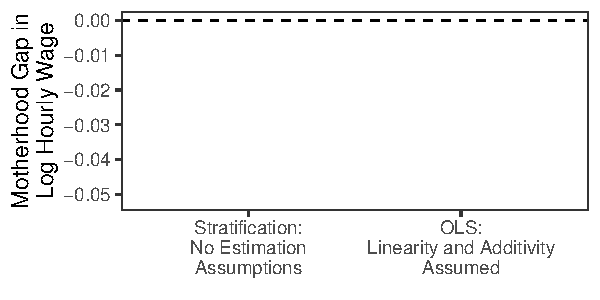
\includegraphics[width = .65\textwidth]{output/slides_motherhood_extremes_0}};
\node<4>[anchor = south] at (.5,.2) {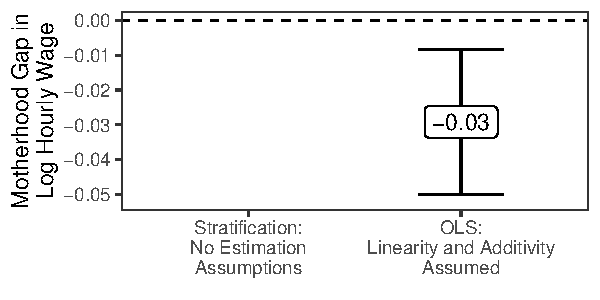
\includegraphics[width = .65\textwidth]{output/slides_motherhood_extremes_1}};
\node<5->[anchor = south] at (.5,.2) {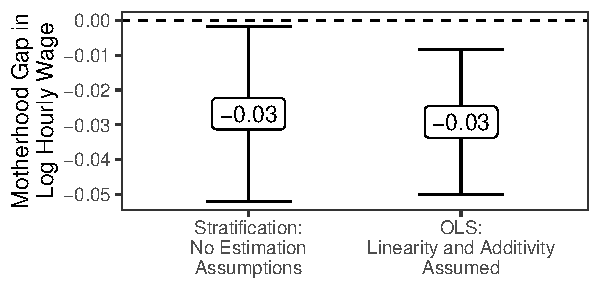
\includegraphics[width = .65\textwidth]{output/slides_motherhood_extremes_2}};
\end{tikzpicture}
\end{frame}

\section{Examples}

\begin{frame}[t]
\headerfigure \vskip .1in
Precise estimands would \bblue{clarify confusion} in the literature \vskip .2in
\begin{tikzpicture}[x = \textwidth, y = 1in]
\node<2->[anchor = west] at (0,0) {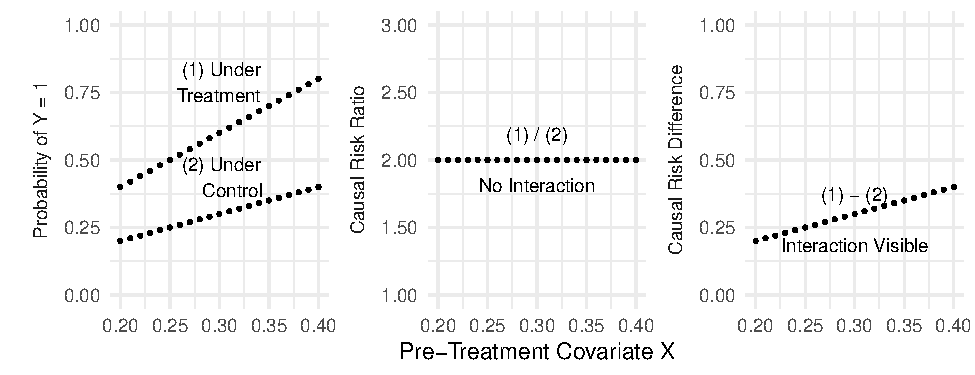
\includegraphics[width = \textwidth]{output/risk_ratio_difference}};
\node<2>[anchor = west] at (.04,-.74) {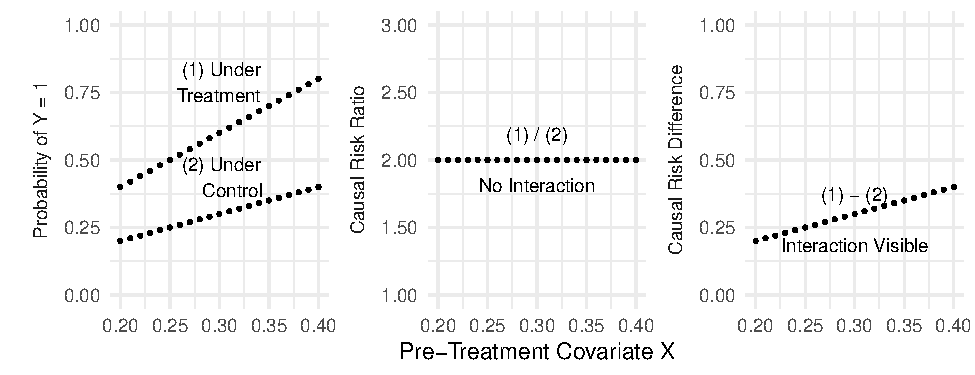
\includegraphics[trim = {2.4in 0in 2in 2.25in}, clip, width = 1.4in]{output/risk_ratio_difference}};
\draw<2>[fill = white, draw = white] (.36,-.65) rectangle (1.05,.8);
\draw<2>[fill = white, draw = white] (.4,-.65) rectangle (.8,-.8);
\draw<3>[fill = white, draw = white] (.69,-.65) rectangle (1.05,.8);
\end{tikzpicture}\vskip .2in
\onslide<5>{
It depends on the \bblue{estimand}
}
\end{frame}
    
    \section{Conclusion}
    
    \begin{frame}[t]
    \headerfigure \vskip .2in
    The \bblue{target tautology} is widespread\\$\rightarrow$ goals are defined by procedures done to data
    \vskip .1in \pause
    Instead, we should \bblue{set the target} nonparametrically\\
    $\rightarrow$ could be approximated by many candidate procedures
    \vskip .1in \pause
    Estimands bring \bblue{benefits} to everyone. \pause
    \begin{itemize}
    \item Estimands help the \bgreen{analyst} to make methodological choices \pause
    \item Estimands help the \bgreen{reviewer} to pinpoint the step where the link to theory breaks down \pause
    \item Estimands help the \bgreen{community} to clarify the contribution of each paper
    \end{itemize}
    \end{frame}
    
    \begin{frame}
\resizebox{\textwidth}{!}{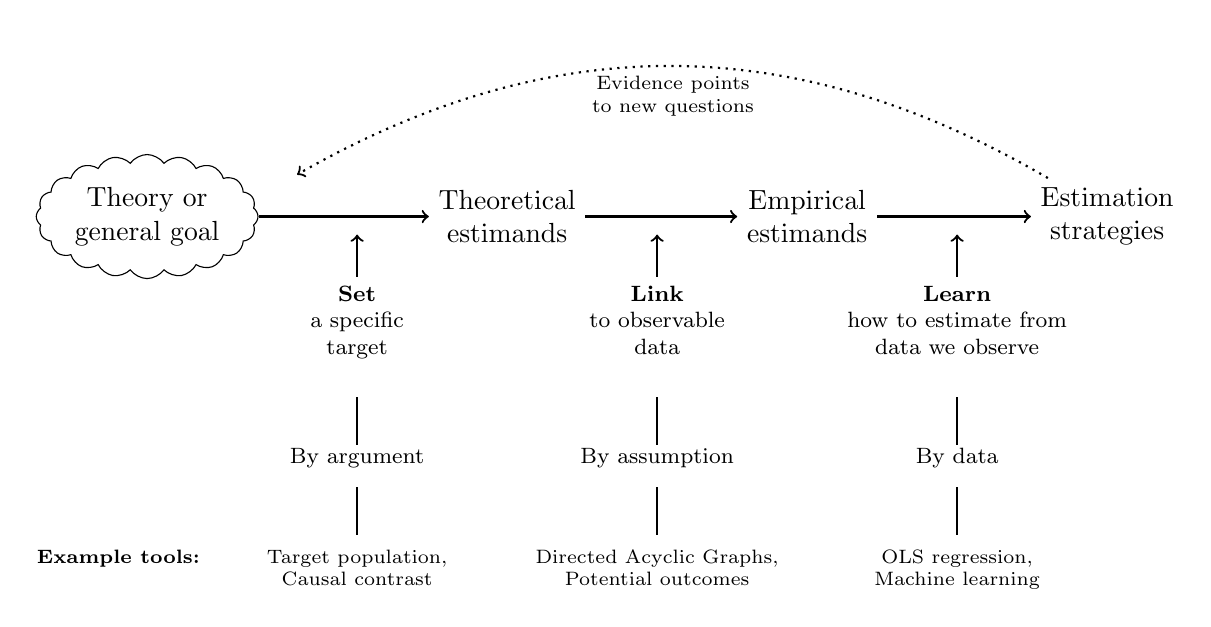
\begin{tikzpicture}[x = 1.5in, y = .3in]
    \node[cloud, draw, align=center, cloud puffs=20,cloud puff arc=110, aspect=2, inner sep=.5mm] (general) at (-.2,0) {Theory or\\general goal};
    \node[align=center] (theoretical) at (1,0) {Theoretical\\estimands};
    \node[align=center] (empirical) at (2,0) {Empirical\\estimands};
    \node[align=center] (estimate) at (3,0) {Estimation\\strategies};
    %%%%%%%%%%
    \node[align=center, font = \footnotesize, anchor = north] (define) at (.5,-1) {\textbf{Set}\\a specific\\target};
    \node[align=center, font = \footnotesize, anchor = north] (identify) at (1.5,-1) {\textbf{Link}\\to observable\\data};
    \node[align=center, font = \footnotesize, anchor = north] (learn) at (2.5,-1) {\textbf{Learn}\\how to estimate from\\data we observe};
    %%%%%%%%%%
    \node[align=center, font = \footnotesize, anchor = north] at (.5,-3.7) {By argument};
    \node[align=center, font = \footnotesize, anchor = north] at (1.5,-3.7) {By assumption};
    \node[align=center, font = \footnotesize, anchor = north] at (2.5,-3.7) {By data};
    %%%%%%%%%%
    %\draw[rounded corners, line width = 1.5pt, gray] (-.2,-6) rectangle (2.85,-7);
    \node[align=center, font = \scriptsize, anchor = north west] at (-.6,-5.4) {\textbf{Example tools:}};
    \node[align=center, font = \scriptsize, anchor = north] at (.5,-5.4) {Target population,\\Causal contrast};
    \node[align=center, font = \scriptsize, anchor = north] at (1.5,-5.4) {Directed Acyclic Graphs,\\Potential outcomes};
    \node[align=center, font = \scriptsize, anchor = north] at (2.5,-5.4) {OLS regression,\\Machine learning};
    %%%%%%%%%%
    \draw[->, thick] (general) -- (theoretical);
    \draw[->, thick] (theoretical) -- (empirical);
    \draw[->, thick] (empirical) -- (estimate);
    \draw[->, thick] (define) -- (.5,-.3);
    \draw[->, thick] (identify) -- (1.5,-.3);
    \draw[->, thick] (learn) -- (2.5,-.3);
    \draw[thick] (.5,-3.8) -- (.5,-3);
    \draw[thick] (1.5,-3.8) -- (1.5,-3);
    \draw[thick] (2.5,-3.8) -- (2.5,-3);
    \draw[thick] (.5,-5.3) -- (.5,-4.5);
    \draw[thick] (1.5,-5.3) -- (1.5,-4.5);
    \draw[thick] (2.5,-5.3) -- (2.5,-4.5);
    % Estimation links back to theory
    \draw[->, thick, dotted] (estimate) to[bend right] node[midway, below, font = \scriptsize, align = center] {Evidence points\\to new questions} (.3,.7);
    \end{tikzpicture}
    } \vskip .2in
    \bref{https://doi.org/10.31235/osf.io/ba67n}{Paper} on SocArxiv.\\
    \bref{https://github.com/ilundberg/replication/tree/master/setting_the_target}{Replication code} on GitHub.\\
    \bref{https://github.com/ilundberg/slides}{Slides} on GitHub.
\end{frame}

\end{document}